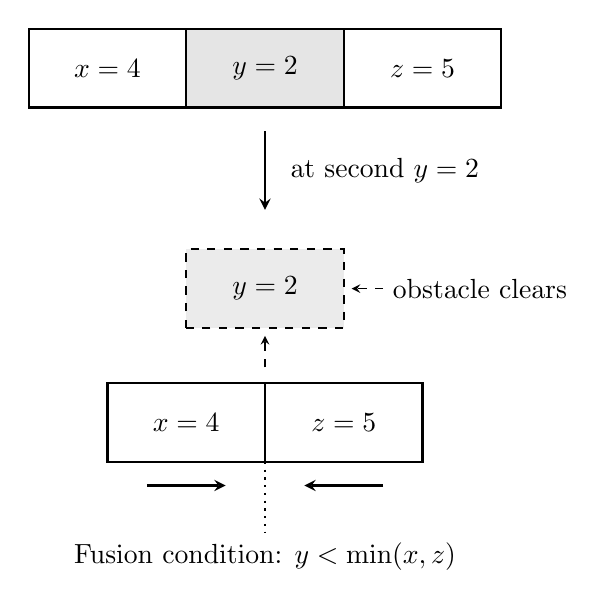
\begin{tikzpicture}[>=stealth]

% Top State: Initial blocks
\gid{blue-left-block}{
    \draw[thick] (0, 3) rectangle (2, 4);
}
\gid{red-middle-block}{
    \draw[thick, fill=black, fill opacity=0.1] (2, 3) rectangle (4, 4);
}
\gid{blue-right-block}{
    \draw[thick] (4, 3) rectangle (6, 4);
}
\gid{labels-blue-lifetimes}{
    \node at (1, 3.5) {$x=4$};
    \node at (5, 3.5) {$z=5$};
}
\gid{label-y}{
    \node at (3, 3.5) {$y=2$};
}

% Transition arrow
\gid{arrow-down}{
    \draw[->, thick] (3, 2.7) -- (3, 1.7);
    \node[right] at (3.2, 2.2) {at second $y=2$};
}

% Bottom State: Vanishing obstacle
\gid{red-vanishing}{
    \draw[thick, dashed, fill=black, fill opacity=0.08] (2, 0.2) rectangle (4, 1.2);
    \node at (3, 0.7) {$y=2$};
    \draw[->, dashed] (3, -0.3) -- (3, 0.1);
}
\gid{label-obstacle-clears}{
    \node[right] (obs) at (4.5, 0.7) {obstacle clears};
    \draw[->, dashed] (obs.west) -- (4.1, 0.7);
}

% Bottom State: Sliding and meeting blocks
\gid{blue-blocks-meeting}{
    \draw[thick] (1, -1.5) rectangle (3, -0.5);
    \node at (2, -1) {$x=4$};
    \draw[->, thick] (1.5, -1.8) -- (2.5, -1.8);
    
    \draw[thick] (3, -1.5) rectangle (5, -0.5);
    \node at (4, -1) {$z=5$};
    \draw[->, thick] (4.5, -1.8) -- (3.5, -1.8);
}

% Annotation for the fusion condition
\gid{condition-annotation}{
    \draw[thick, dotted] (3, -1.5) -- (3, -2.4);
    \node[below] at (3, -2.4) {Fusion condition: $y < \min(x, z)$};
}

\end{tikzpicture}